%!TEX root = ../../ClassicThesis.tex
%-------------------------------------------------------------------------------
\section{Introduction}
%-------------------------------------------------------------------------------

%-------------------------------------------------------------------------------
\section{Results}
%-------------------------------------------------------------------------------

%-------------------------------------------------------------------------------
\subsection{Signal and Noise Correlation}

\marginpar{Take text from supplemental materials for paper, but here with the addition of phase correlating with itself and with power.}

\begin{figure}[htb]
    \centering
    \subfloat[Signal correlation\label{fig:lam_signal_corr_depth}]{
        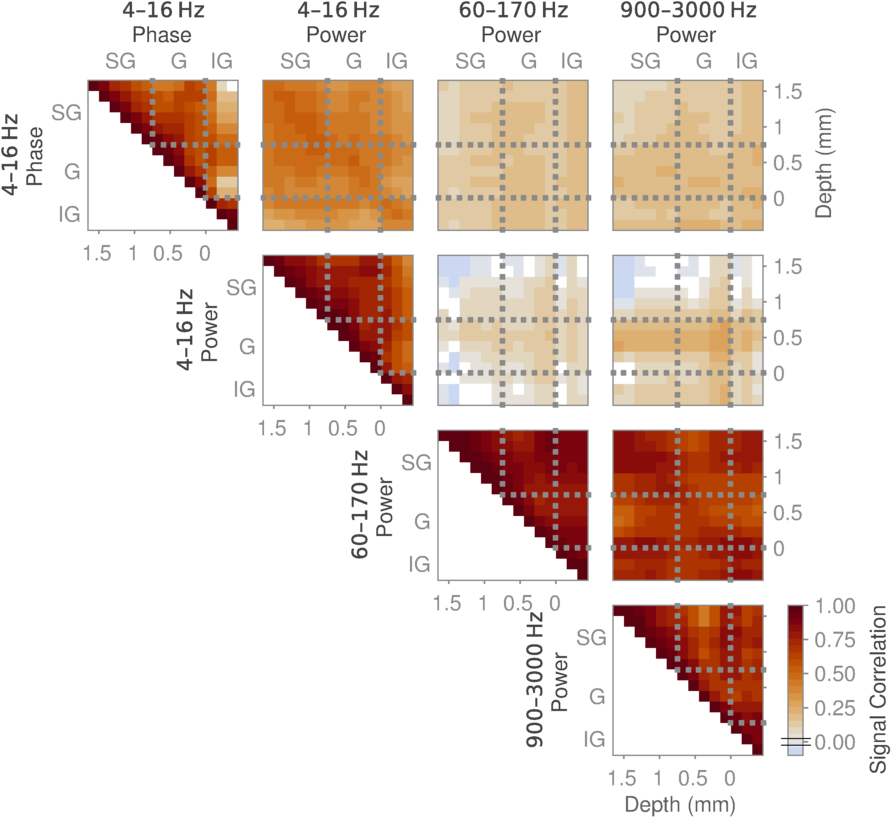
\includegraphics[scale=.5]{noisesigcorr/bndflt4-signal-avg_paper.png}
}
    \\
    \subfloat[Noise correlation\label{fig:lam_noise_corr_depth}]{
        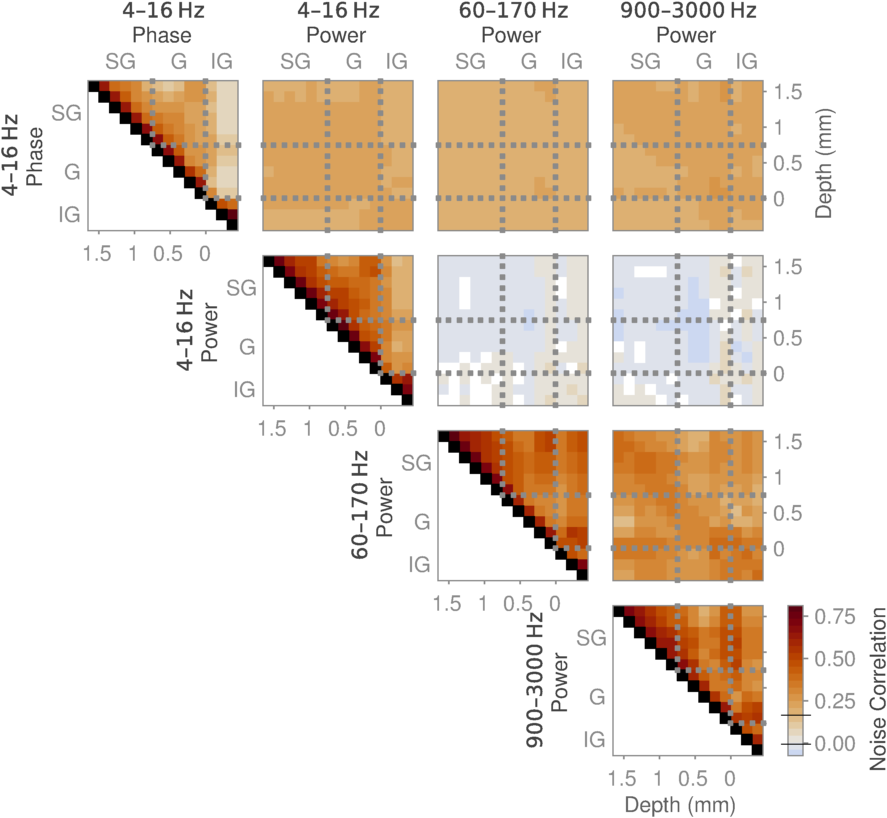
\includegraphics[scale=.5]{noisesigcorr/bndflt4-noise-avg_paper.png}
}
    \caption{
\protect\subref{fig:lam_signal_corr_depth}:~Signal correlation.
\protect\subref{fig:lam_noise_corr_depth}:~Noise correlation.
}
\label{fig:lam_noisesignal_corr_depth}
\end{figure}


\begin{figure}[htb]
    \centering
    \hspace*{\fill}
    \subfloat[Signal correlation\label{fig:lam_signal_corr_phase}]{
        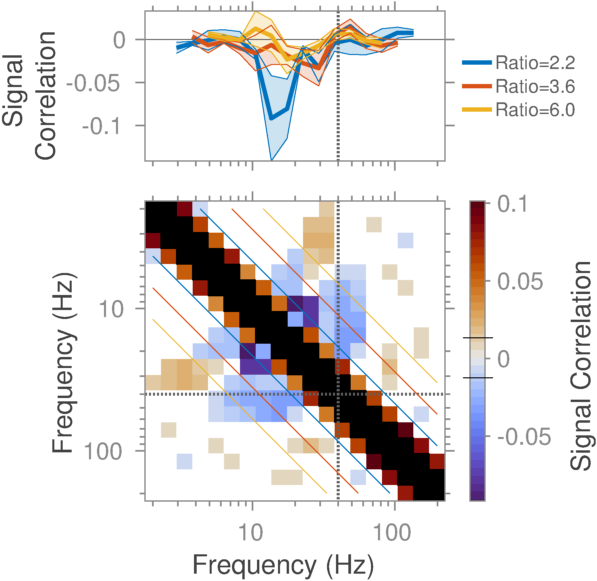
\includegraphics[scale=.45]{noisesigcorr/cxsfrq-signal-phase-phase-avg-log.png}
}
    \hspace*{\fill}\hspace{.2cm}\hspace*{\fill}
    \subfloat[Noise correlation\label{fig:lam_noise_corr_phase}]{
        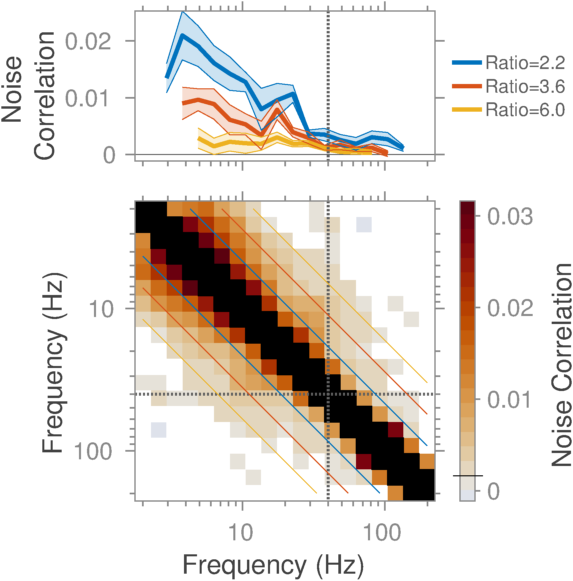
\includegraphics[scale=.45]{noisesigcorr/cxsfrq-noise-phase-phase-avg-log.png}
}
    \hspace*{\fill}
    \caption{Phase correlation
\protect\subref{fig:lam_signal_corr_phase}:~Signal correlation.
\protect\subref{fig:lam_noise_corr_phase}:~Noise correlation.
}
\label{fig:lam_noisesignal_corr_phase}
\end{figure}

\begin{figure}[htb]
    \centering
    \hspace*{\fill}
    \subfloat[Signal correlation\label{fig:lam_signal_corr_phase_power}]{
        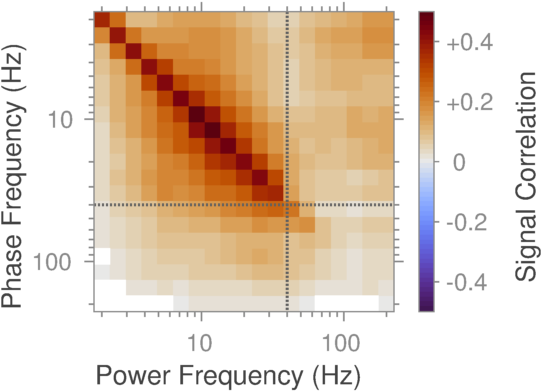
\includegraphics[scale=.45]{noisesigcorr/cxsfrq-signal-phase-power-avg-log.png}
}
    \hspace*{\fill}\hspace{.2cm}\hspace*{\fill}
    \subfloat[Noise correlation\label{fig:lam_noise_corr_phase_power}]{
        %\includegraphics[scale=.45]{noisesigcorr/cxsfrq-noise-phase-power-avg-log.png}
        <code running>
}
    \hspace*{\fill}
    \caption{Phase correlation with power
\protect\subref{fig:lam_signal_corr_phase_power}:~Signal correlation.
\protect\subref{fig:lam_noise_corr_phase_power}:~Noise correlation.
}
\label{fig:lam_noisesignal_corr_phase_power}
\end{figure}

Circular statistics were computed using the CircStat toolbox \citep{Berens2009}.

%-------------------------------------------------------------------------------
\subsection{Phase correlation, \SIrange{4}{16}{Hz}}

Circular statistics were computed using the CircStat toolbox \citep{Berens2009}.

\begin{figure}[htb]
    \centering
    \hspace*{\fill}
    \subfloat[Movie driven\label{fig:lam_phasestats_alpha_line_csd_movie}]{
        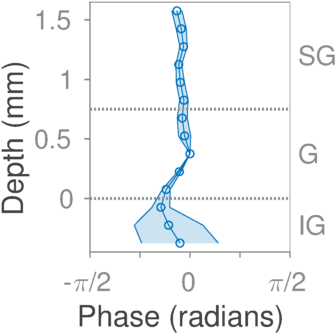
\includegraphics[scale=.45]{phasestats/movie1_Csd_phs4-16_dPhsTracebnd_5mean.png}
}
    \hspace*{\fill}\hspace{.2cm}\hspace*{\fill}
    \subfloat[Spontaneous\label{fig:lam_phasestats_alpha_line_csd_spont}]{
        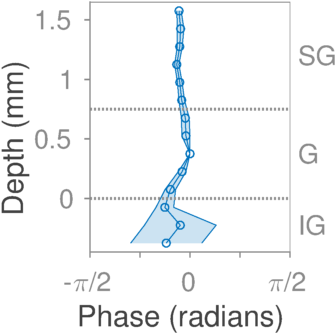
\includegraphics[scale=.45]{phasestats/spont_Csd_phs4-16_dPhsTracebnd_5mean.png}
}
    \hspace*{\fill}
    \caption{Phase correlation, \SIrange{4}{16}{Hz}.
\protect\subref{fig:lam_phasestats_alpha_line_csd_movie}:~Movie driven.
\protect\subref{fig:lam_phasestats_alpha_line_csd_spont}:~Spontaneous.
}
\label{fig:lam_phasestats_alpha_line_csd}
\end{figure}


\begin{figure}[htb]
    \centering
    \hspace*{\fill}
    \subfloat[Movie driven\label{fig:lam_phasestats_alpha_hist_csd_movie}]{
        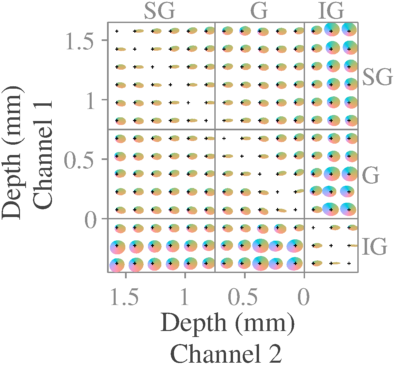
\includegraphics[scale=.45]{phasestats/movie1_Csd_phs4-16_dPhs_hist_5mean.png}
}
    \hspace*{\fill}\hspace{.2cm}\hspace*{\fill}
    \subfloat[Spontaneous\label{fig:lam_phasestats_alpha_hist_csd_spont}]{
        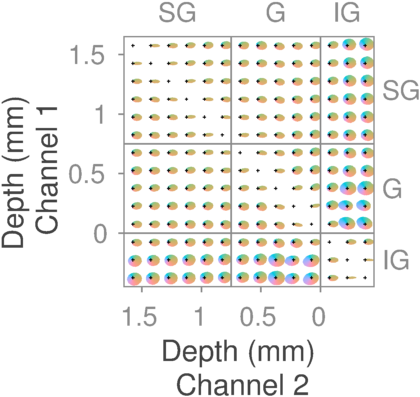
\includegraphics[scale=.45]{phasestats/spont_Csd_phs4-16_dPhs_hist_5mean.png}
}
    \hspace*{\fill}
    \caption{Phase correlation, \SIrange{4}{16}{Hz}.
\protect\subref{fig:lam_phasestats_alpha_hist_csd_movie}:~Movie driven.
\protect\subref{fig:lam_phasestats_alpha_hist_csd_spont}:~Spontaneous.
}
\label{fig:lam_phasestats_alpha_hist_csd}
\end{figure}


\begin{figure}[htb]
    \centering
    \hspace*{\fill}
    \subfloat[Movie driven\label{fig:lam_phasestats_alpha_combo_csd_movie}]{
        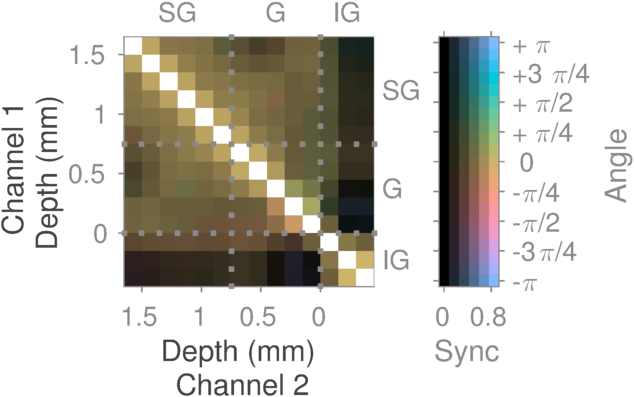
\includegraphics[scale=.45]{phasestats/movie1_Csd_phs4-16_dPhs_combo_5mean.png}
}
    \hspace*{\fill}\hspace{.2cm}\hspace*{\fill}
    \subfloat[Spontaneous\label{fig:lam_phasestats_alpha_combo_csd_spont}]{
        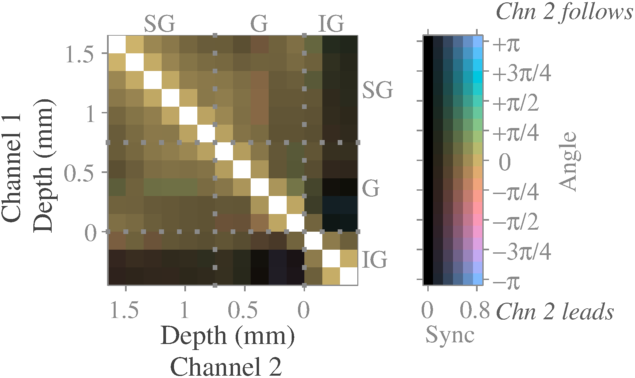
\includegraphics[scale=.45]{phasestats/spont_Csd_phs4-16_dPhs_combo_5mean.png}
}
    \hspace*{\fill}
    \caption{Phase correlation, showing phase offset and synchronicity \SIrange{4}{16}{Hz}.
\protect\subref{fig:lam_phasestats_alpha_combo_csd_movie}:~Movie driven.
\protect\subref{fig:lam_phasestats_alpha_combo_csd_spont}:~Spontaneous.
}
\label{fig:lam_phasestats_alpha_combo_csd}
\end{figure}


\begin{figure}[htb]
    \centering
    \hspace*{\fill}
    \subfloat[Movie driven\label{fig:lam_phasestats_alpha_summary_csd_movie}]{
        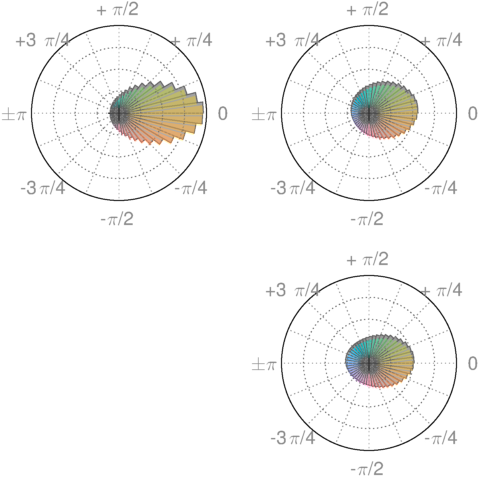
\includegraphics[scale=.45]{phasestats/movie1_Csd_simplephs4-16_dPhs_hist.png}
}
    \hspace*{\fill}\hspace{.2cm}\hspace*{\fill}
    \subfloat[Spontaneous\label{fig:lam_phasestats_alpha_summary_csd_spont}]{
        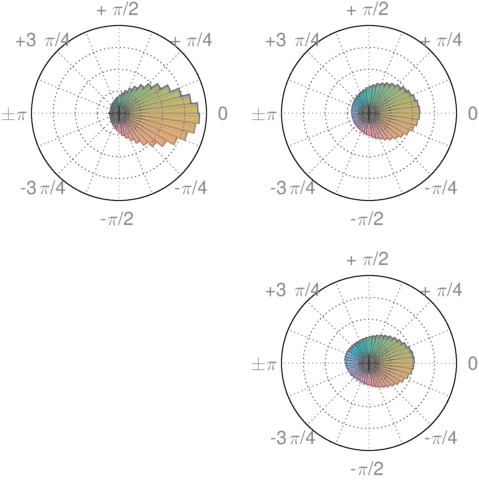
\includegraphics[scale=.45]{phasestats/spont_Csd_simplephs4-16_dPhs_hist.png}
}
    \hspace*{\fill}
    \caption{Phase correlation, summary by region, \SIrange{4}{16}{Hz}.
\protect\subref{fig:lam_phasestats_alpha_summary_csd_movie}:~Movie driven.
\protect\subref{fig:lam_phasestats_alpha_summary_csd_spont}:~Spontaneous.
}
\label{fig:lam_phasestats_alpha_summary_csd}
\end{figure}

%-------------------------------------------------------------------------------
\subsection{Phase correlation, \SIrange{60}{170}{Hz}}

Circular statistics were computed using the CircStat toolbox \citep{Berens2009}.

\begin{figure}[htb]
    \centering
    \hspace*{\fill}
    \subfloat[Movie driven\label{fig:lam_phasestats_gamma_line_csd_movie}]{
        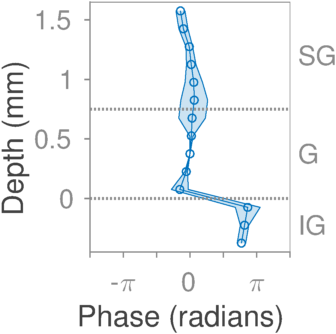
\includegraphics[scale=.45]{phasestats/movie1_Csd_phs60-170_dPhsTracebnd_5mean.png}
}
    \hspace*{\fill}\hspace{.2cm}\hspace*{\fill}
    \subfloat[Spontaneous\label{fig:lam_phasestats_gamma_line_csd_spont}]{
        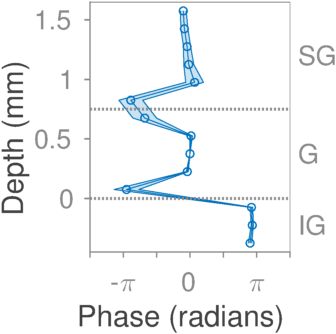
\includegraphics[scale=.45]{phasestats/spont_Csd_phs60-170_dPhsTracebnd_5mean.png}
}
    \hspace*{\fill}
    \caption{Phase correlation, \SIrange{60}{170}{Hz}.
\protect\subref{fig:lam_phasestats_gamma_line_csd_movie}:~Movie driven.
\protect\subref{fig:lam_phasestats_gamma_line_csd_spont}:~Spontaneous.
}
\label{fig:lam_phasestats_gamma_line_csd}
\end{figure}


\begin{figure}[htb]
    \centering
    \hspace*{\fill}
    \subfloat[Movie driven\label{fig:lam_phasestats_gamma_hist_csd_movie}]{
        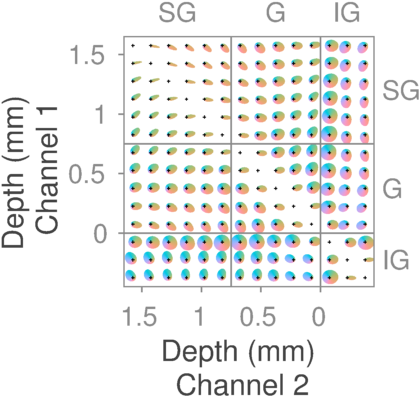
\includegraphics[scale=.45]{phasestats/movie1_Csd_phs60-170_dPhs_hist_5mean.png}
}
    \hspace*{\fill}\hspace{.2cm}\hspace*{\fill}
    \subfloat[Spontaneous\label{fig:lam_phasestats_gamma_hist_csd_spont}]{
        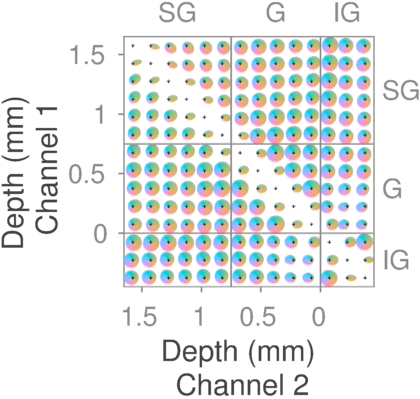
\includegraphics[scale=.45]{phasestats/spont_Csd_phs60-170_dPhs_hist_5mean.png}
}
    \hspace*{\fill}
    \caption{Phase correlation, \SIrange{60}{170}{Hz}.
\protect\subref{fig:lam_phasestats_gamma_hist_csd_movie}:~Movie driven.
\protect\subref{fig:lam_phasestats_gamma_hist_csd_spont}:~Spontaneous.
}
\label{fig:lam_phasestats_gamma_hist_csd}
\end{figure}


\begin{figure}[htb]
    \centering
    \hspace*{\fill}
    \subfloat[Movie driven\label{fig:lam_phasestats_gamma_combo_csd_movie}]{
        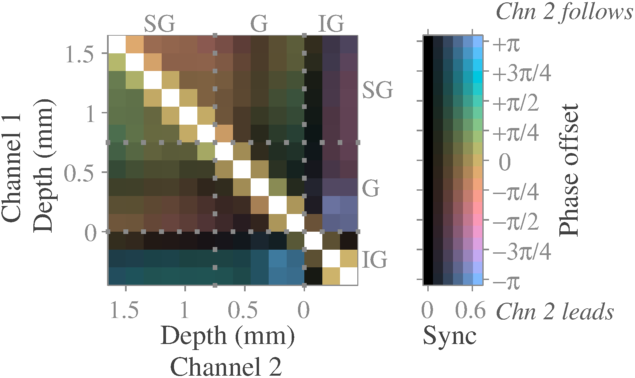
\includegraphics[scale=.45]{phasestats/movie1_Csd_phs60-170_dPhs_combo_5mean.png}
}
    \hspace*{\fill}\hspace{.2cm}\hspace*{\fill}
    \subfloat[Spontaneous\label{fig:lam_phasestats_gamma_combo_csd_spont}]{
        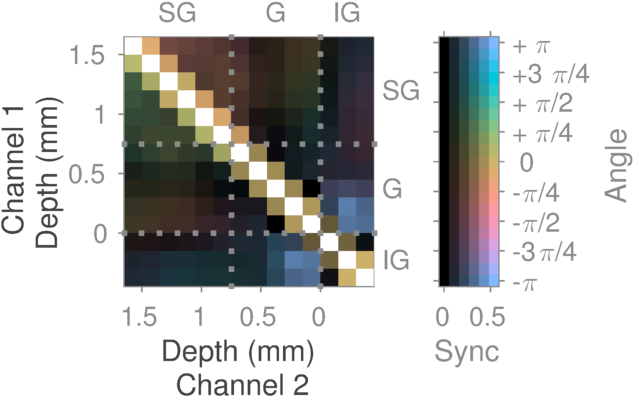
\includegraphics[scale=.45]{phasestats/spont_Csd_phs60-170_dPhs_combo_5mean.png}
}
    \hspace*{\fill}
    \caption{Phase correlation, showing phase offset and synchronicity \SIrange{60}{170}{Hz}.
\protect\subref{fig:lam_phasestats_gamma_combo_csd_movie}:~Movie driven.
\protect\subref{fig:lam_phasestats_gamma_combo_csd_spont}:~Spontaneous.
}
\label{fig:lam_phasestats_gamma_combo_csd}
\end{figure}


\begin{figure}[htb]
    \centering
    \hspace*{\fill}
    \subfloat[Movie driven\label{fig:lam_phasestats_gamma_summary_csd_movie}]{
        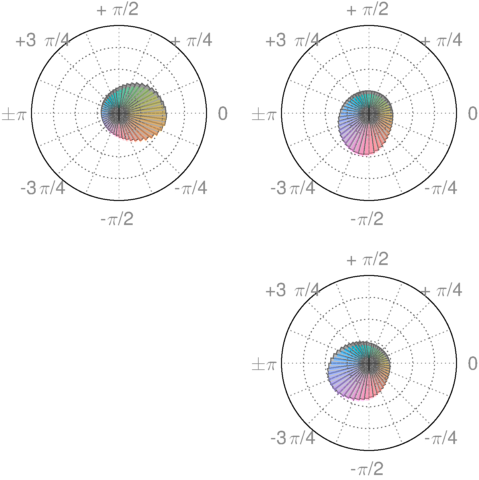
\includegraphics[scale=.45]{phasestats/movie1_Csd_simplephs60-170_dPhs_hist.png}
}
    \hspace*{\fill}\hspace{.2cm}\hspace*{\fill}
    \subfloat[Spontaneous\label{fig:lam_phasestats_gamma_summary_csd_spont}]{
        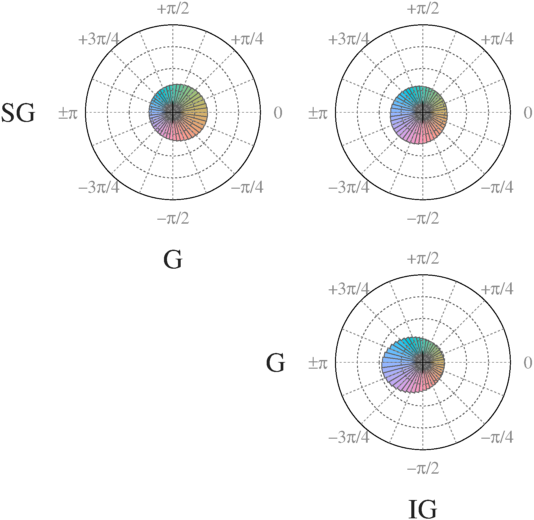
\includegraphics[scale=.45]{phasestats/spont_Csd_simplephs60-170_dPhs_hist.png}
}
    \hspace*{\fill}
    \caption{Phase correlation, summary by region, \SIrange{60}{170}{Hz}.
\protect\subref{fig:lam_phasestats_gamma_summary_csd_movie}:~Movie driven.
\protect\subref{fig:lam_phasestats_gamma_summary_csd_spont}:~Spontaneous.
}
\label{fig:lam_phasestats_gamma_summary_csd}
\end{figure}


%-------------------------------------------------------------------------------
\subsection{Stimulus information contained in phase}

\begin{figure}[htb]
    \centering
    \subfloat[\ac{LFP}\label{fig:lam_phase_info_lfp}]{
        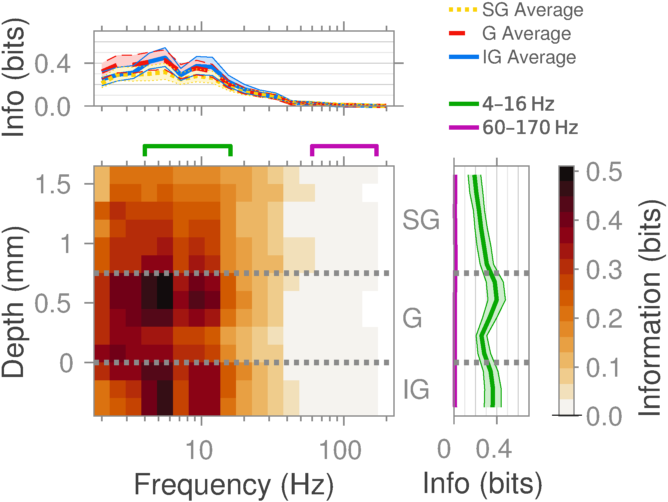
\includegraphics[scale=.5]{phaseinfo/fig3set-info-Csd-phase-straightnanmean-compzonescb-legend.png}
}
    \\
    \subfloat[\ac{CSD}\label{fig:lam_phase_info_csd}]{
        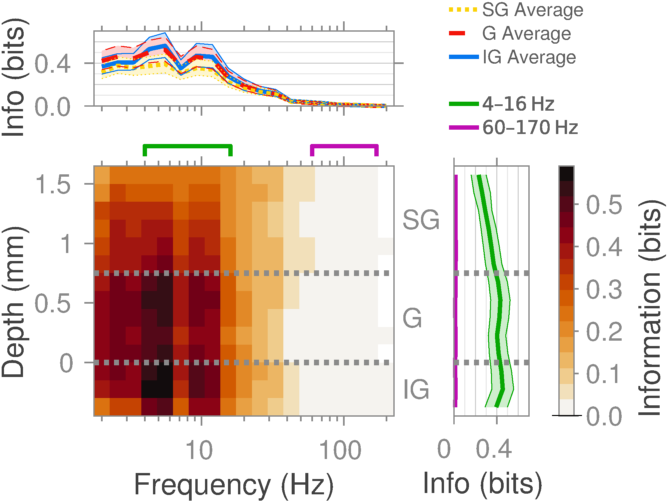
\includegraphics[scale=.5]{phaseinfo/fig3set-info-Cln-phase-straightnanmean-compzonescb-legend.png}
}
    \caption{
Information about the stimulus contained in the phase of the extracellular neural signal, as a function of frequency. Mean of 6 sessions.
\protect\subref{fig:lam_phase_info_lfp}:~\ac{LFP}.
\protect\subref{fig:lam_phase_info_csd}:~\ac{CSD}.
}
\label{fig:lam_phase_info}
\end{figure}


\begin{figure}[htb]
    \centering
    \hspace*{\fill}
    \subfloat[\sesname{H05391}\label{fig:lam_phase_info_lfp_H05391}]{
        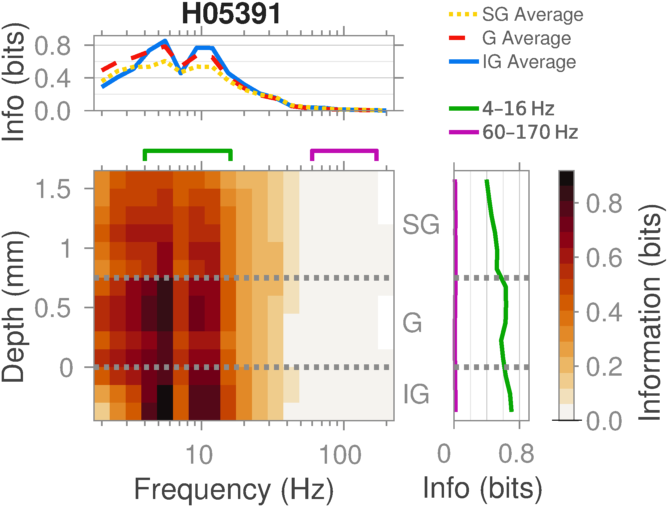
\includegraphics[scale=.4]{phaseinfo/fig3set-info-Cln-phase-H05391-compzonescb-legend.png}
}
    \hspace*{\fill}\hspace{.2cm}\hspace*{\fill}
    \subfloat[\sesname{H05nm9}\label{fig:lam_phase_info_lfp_H05nm9}]{
        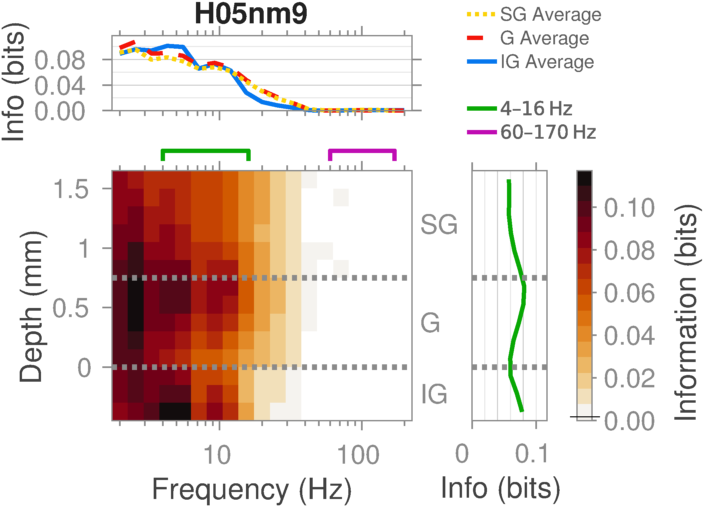
\includegraphics[scale=.4]{phaseinfo/fig3set-info-Cln-phase-H05nm9-compzonescb-legend.png}
}
    \hspace*{\fill}
    \\
    \hspace*{\fill}
    \subfloat[\sesname{H05nm7}\label{fig:lam_phase_info_lfp_H05nm7}]{
        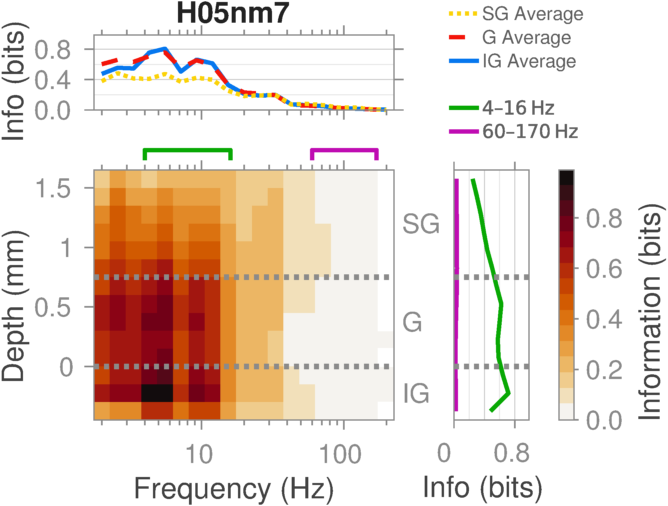
\includegraphics[scale=.4]{phaseinfo/fig3set-info-Cln-phase-H05nm7-compzonescb-legend.png}
}
    \hspace*{\fill}\hspace{.2cm}\hspace*{\fill}
    \subfloat[\sesname{E07nm1}\label{fig:lam_phase_info_lfp_E07nm1}]{
        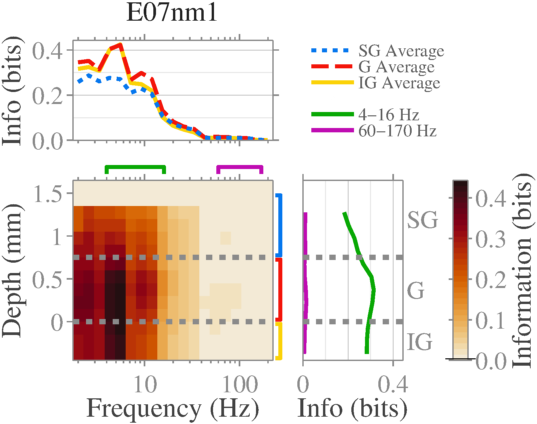
\includegraphics[scale=.4]{phaseinfo/fig3set-info-Cln-phase-E07nm1-compzonescb-legend.png}
}
    \hspace*{\fill}
    \\
    \hspace*{\fill}
    \subfloat[\sesname{F10nm1}\label{fig:lam_phase_info_lfp_F10nm1}]{
        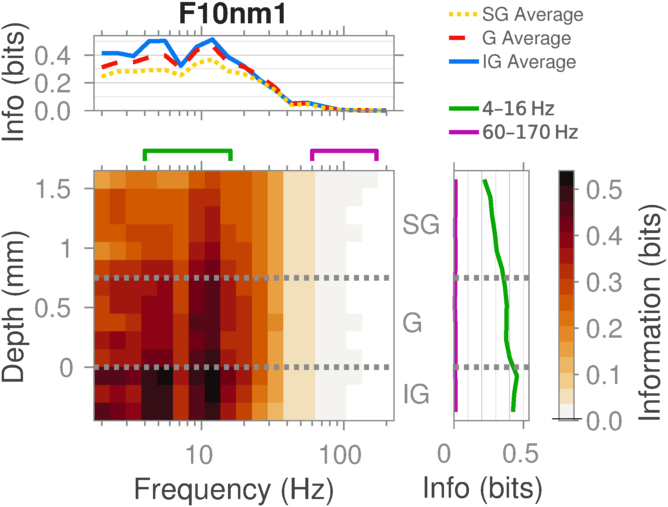
\includegraphics[scale=.4]{phaseinfo/fig3set-info-Cln-phase-F10nm1-compzonescb-legend.png}
}
    \hspace*{\fill}\hspace{.2cm}\hspace*{\fill}
    \subfloat[\sesname{J10nm1}\label{fig:lam_phase_info_lfp_J10nm1}]{
        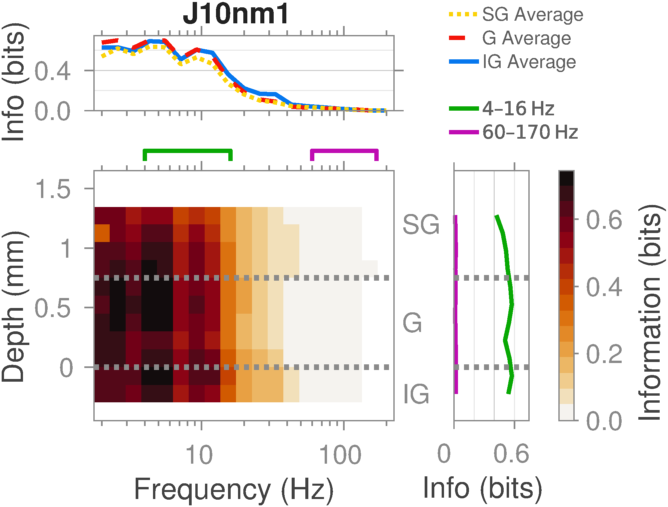
\includegraphics[scale=.4]{phaseinfo/fig3set-info-Cln-phase-J10nm1-compzonescb-legend.png}
}
    \hspace*{\fill}
    \caption{
Information about the stimulus contained in the phase of the \ac{LFP}, as a function of frequency, by session.
}
\label{fig:lam_phase_info}
\end{figure}


\begin{figure}[htb]
    \centering
    \hspace*{\fill}
    \subfloat[\sesname{H05391}\label{fig:lam_phase_info_csd_H05391}]{
        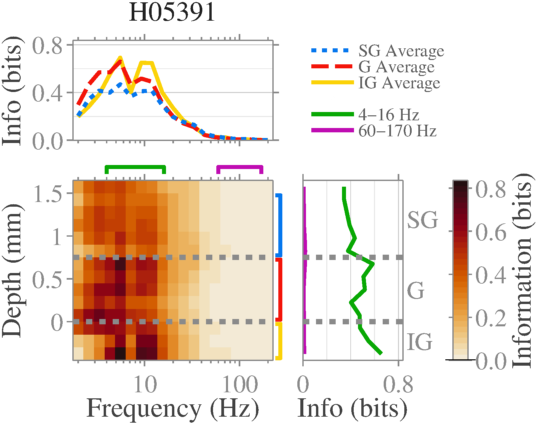
\includegraphics[scale=.4]{phaseinfo/fig3set-info-Csd-phase-H05391-compzonescb-legend.png}
}
    \hspace*{\fill}\hspace{.2cm}\hspace*{\fill}
    \subfloat[\sesname{H05nm9}\label{fig:lam_phase_info_csd_H05nm9}]{
        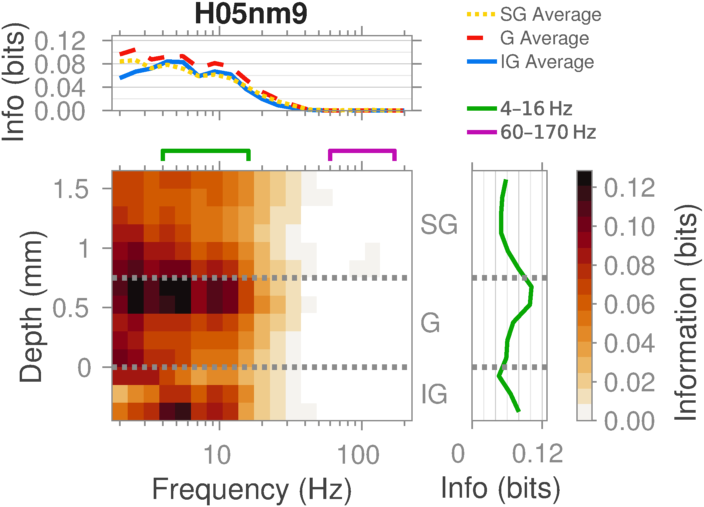
\includegraphics[scale=.4]{phaseinfo/fig3set-info-Csd-phase-H05nm9-compzonescb-legend.png}
}
    \hspace*{\fill}
    \\
    \hspace*{\fill}
    \subfloat[\sesname{H05nm7}\label{fig:lam_phase_info_csd_H05nm7}]{
        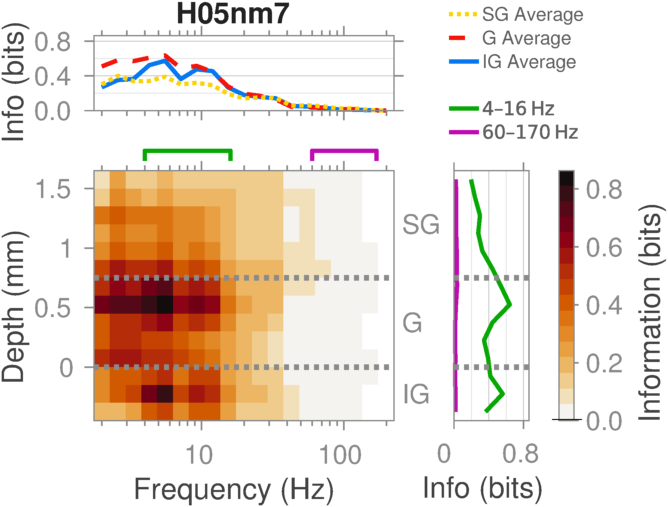
\includegraphics[scale=.4]{phaseinfo/fig3set-info-Csd-phase-H05nm7-compzonescb-legend.png}
}
    \hspace*{\fill}\hspace{.2cm}\hspace*{\fill}
    \subfloat[\sesname{E07nm1}\label{fig:lam_phase_info_csd_E07nm1}]{
        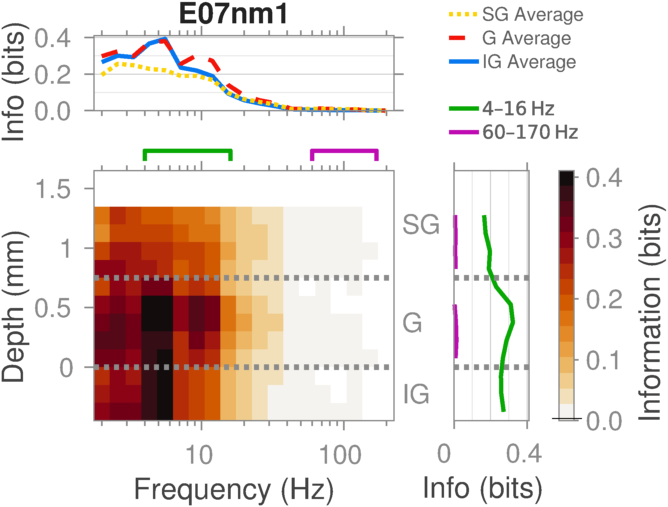
\includegraphics[scale=.4]{phaseinfo/fig3set-info-Csd-phase-E07nm1-compzonescb-legend.png}
}
    \hspace*{\fill}
    \\
    \hspace*{\fill}
    \subfloat[\sesname{F10nm1}\label{fig:lam_phase_info_csd_F10nm1}]{
        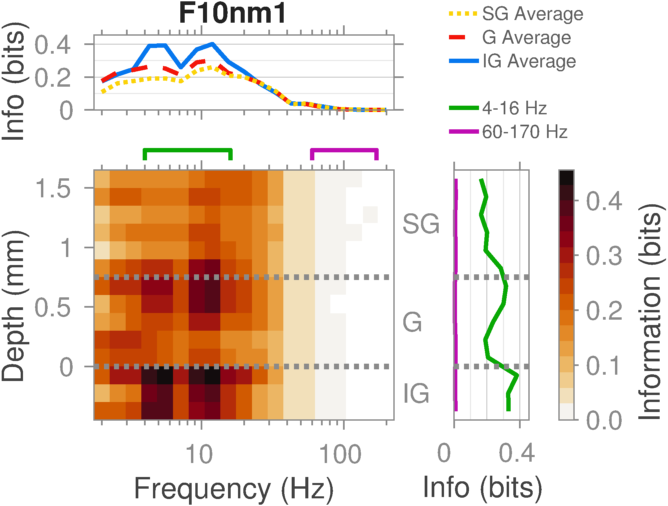
\includegraphics[scale=.4]{phaseinfo/fig3set-info-Csd-phase-F10nm1-compzonescb-legend.png}
}
    \hspace*{\fill}\hspace{.2cm}\hspace*{\fill}
    \subfloat[\sesname{J10nm1}\label{fig:lam_phase_info_csd_J10nm1}]{
        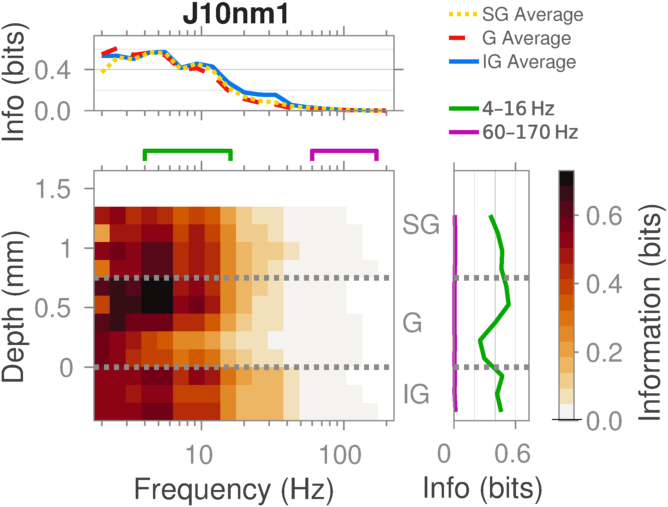
\includegraphics[scale=.4]{phaseinfo/fig3set-info-Csd-phase-J10nm1-compzonescb-legend.png}
}
    \hspace*{\fill}
    \caption{
Information about the stimulus contained in the phase of the \ac{CSD}, as a function of frequency, by session.
}
\label{fig:lam_phase_info}
\end{figure}


%-------------------------------------------------------------------------------
\subsection{Redundancy}

\subsubsection{Cross channel}

\begin{figure}[htb]
    \centering
    \subfloat[\label{fig:lam_phase_cxchn_info_red}]{
        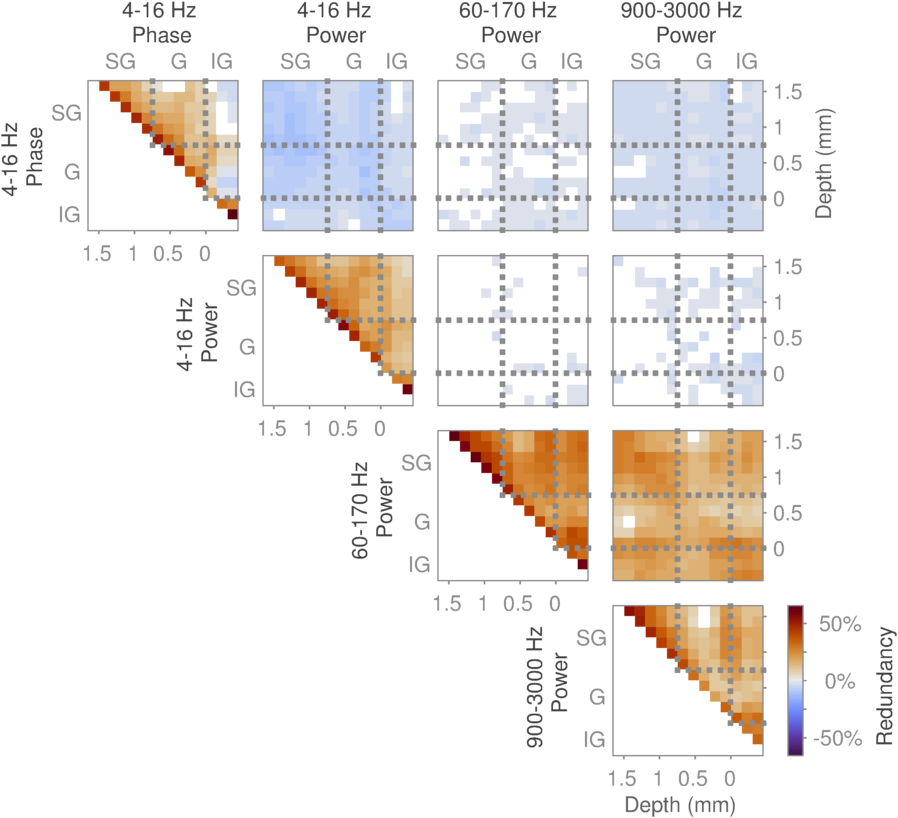
\includegraphics[scale=.5]{phaseredundancy/bndflt4-PCred-none-avg-lag=0s_paper.png}
}
    \\
    \subfloat[\label{fig:lam_phase_cxchn_info_red_bar}]{
        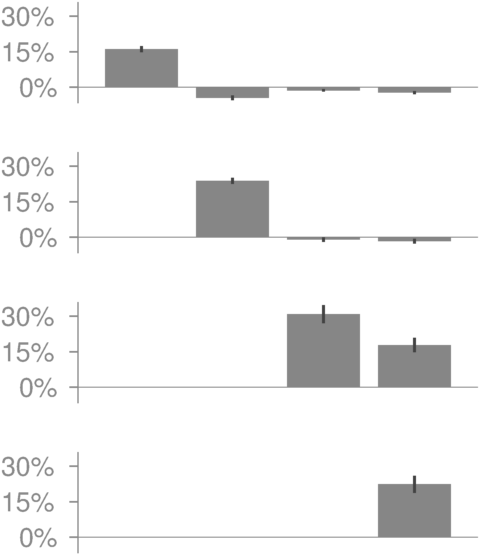
\includegraphics[scale=.5]{phaseredundancy/bndflt-barplot4_PCred-none-avg_lag=0s_paper.png}
}
    \caption{Redundancy of bands across channels.
}
\label{fig:lam_phase_cxchn_info_red_overall}
\end{figure}


\begin{figure}[htb]
    \centering
    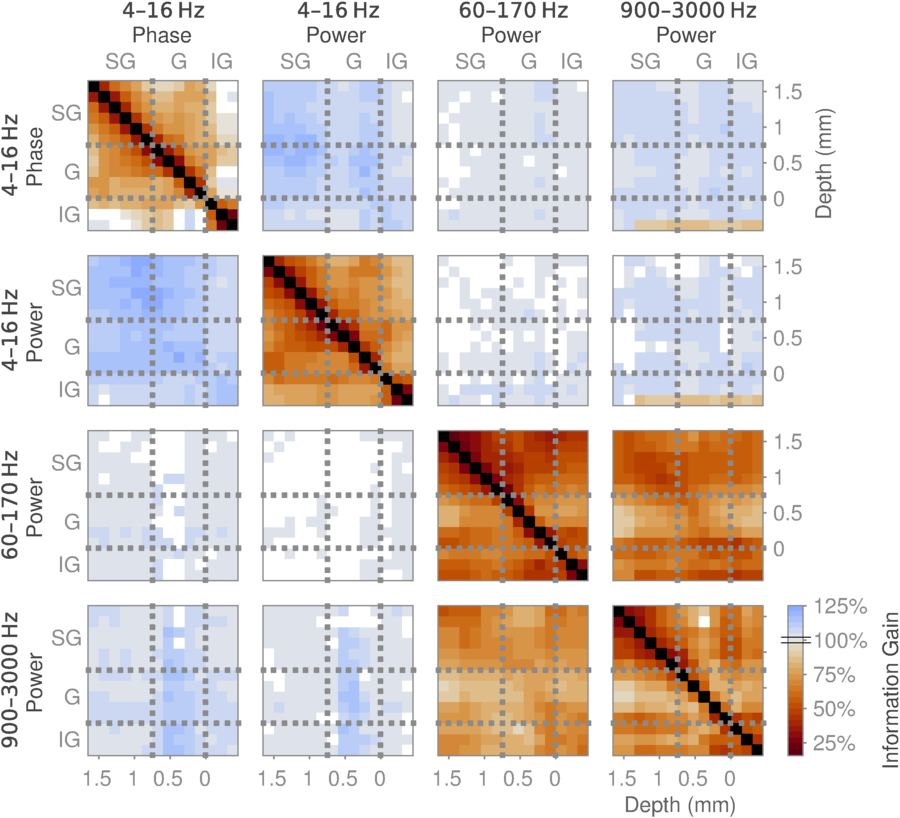
\includegraphics[scale=.5]{phaseredundancy/bndflt4-PCgain-i2d2-none-avg-lag=0s_paper.png}
    \caption{Information gain between bands across channels.
}
\label{fig:lam_phase_cxchn_info_gain}
\end{figure}


%-------------------------------------------------------------------------------
\section{Discussion}
%-------------------------------------------------------------------------------
